\documentclass[a4paper,11pt]{article}
\usepackage{latexsym}
\usepackage[english,polish]{babel}
\usepackage[utf8]{inputenc} 
\usepackage[MeX]{polski}
\usepackage{nicefrac}
\usepackage{graphicx}

\author{Patryk Olejniczak 114989\\ Dawid Wiśniewski 116912 \\ Damian Jackowski 134496}

\title{MMDS Challenge\\
\large{{\bf Raport I}  }} 

\date{24 listopada 2017}

\begin{document}

\maketitle 

\section{Wstęp}
Niniejszy raport został przygotowany na przedmiot Projekt eksploracji danych. Celem niniejszego raportu jest zapoznanie się z danymi konkursowymi. W związku z tym przygotowaliśmy oraz omówiliśmy wykresy kilka wybranych wykresów. Są to m.in. wykresy:
\begin{itemize}
\item histogramy liczby wyświetleń i sprzedaży
\item wykres popularności zapytań w poszczególnych miesiącach
\item histogramy sprzedaży w wybranych kategoriach zależnie od sezonu
\end{itemize}

\section{Omówienie wykresów}
Niniejszy rozdział jest poświęcony szczegółowej analizie wykresów.

\subsection{Histogram liczby wyświetleń}
Rysunek \ref{fig:adsViewsNumber} przedstawia histogram liczby wyświetleń. Na wykresie zobrazowano jak liczba wyświetleń rozkładała się względem liczby ogłoszeń. Ze względu na duże różnice zastosowaliśmy dwie skale - do niebieskich elementów wykresu odnosi się lewa skala, a do czerwonych prawa. Na osi pionowej umieściliśmy liczbę ogłoszeń, a na osi poziomej liczbę wyświetleń dla danej grupy ogłoszeń.

Z wykresu możemy się dowiedzieć, że np. prawie 1900000 ogłoszeń miało mniej niż 2000 wyświetleń (niebieska kropka z lewej strony rysunku). Z kolei około 2100 do 2200 ogłoszeń odnotowało niewiele ponad 2000 wyświetleń (pierwszy od lewej czerwony punkt). Idąc dalej w prawo widzimy, że liczba ogłoszeń gwałtownie spada wraz ze wzrostem liczby wyświetleń.

Powyższa obserwacja doprowadziła nas do kilku wniosków. Po pierwsze widać, że tylko niewielki odsetek ogłoszeń ma ponad 4000 wyświetleń. Na podstawie tego histogramu możemy przypuszczać, że zdecydowana większość ogłoszeń ma niewielką liczbę wyświetleń. To może być spowodowane albo słabą jakością większości ogłoszeń (tzn. że  wiele ogłoszeń nie jest wystarczająco atrakcyjna, żeby zainteresować większą liczbę użytkowników). Z drugiej strony może być też tak, że te najatrakcyjniejsze ogłoszenia są szybko zdejmowane z portalu ze względu na to, że szybko znajdują one nabywców. Myślimy jednak, że ten drugi przypadek dotyczy bardzo niewielu spośród wszystkich ogłoszeń. Większość prawdopodobnie stanowią ogłoszenia mało atrakcyjne.

W takim razie co sprawia, że niektóre ogłoszenia osiągają tak dużo wyświetleń? Wiele z nich jest na portalu przez bardzo długi czas co oznacza, że użytkownicy mają dużo czasu, aby je wyświetlić.

\begin{figure}[!ht]
\centering
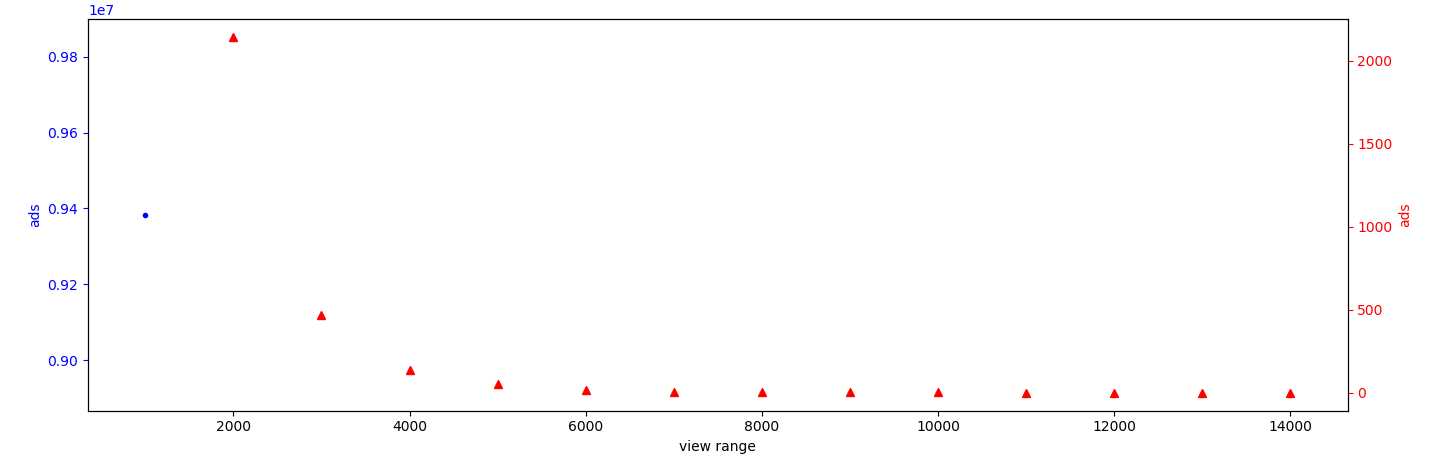
\includegraphics[width=1.0\textwidth]{images/liczba_ogloszen_Liczba_wyswietlen.png}
\caption{\label{fig:adsViewsNumber} histogram liczby ogłoszeń}
\end{figure}

\subsection{Histogram liczby sprzedanych}
Na rysunku \ref{fig:soldNumber} zaprezentowano liczbę sprzedanych przedmiotów w poszczególnych miesiącach. Oś X to nazwy plików odpowiadające poszczególnym miesiącom, a oś Y liczba ogłoszeń zakończonych sprzedażą w danym miesiącu. Widać tutaj wyraźnie, że najwięcej udanych transakcji odbywa się w listopadzie, następnie liczba ta stopniowo spada by w sierpniu osiągnąć poziom trzy razy niższy niż podczas miesiąca z najwyższą liczną sprzedanych przedmiotów. Jest to najniższy poziom w całym roku. Następnie od września notujemy wzrost sprzedaży. Na wykresie pominęliśmy miesiąc październik ze względu na problemy ze sparsowaniem pliku.

\begin{figure}[!ht]
\centering
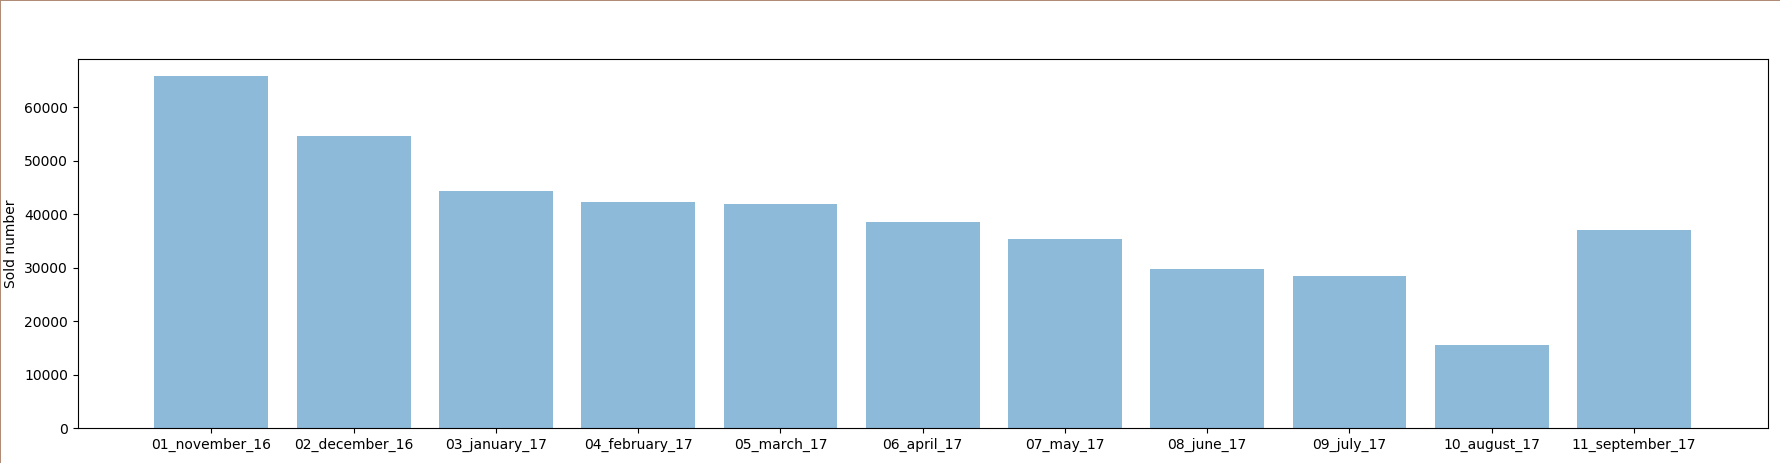
\includegraphics[width=1.0\textwidth]{images/sold_number.png}
\caption{\label{fig:soldNumber} Liczba sprzedaży w poszczególnych miesiącach}
\end{figure}

\subsection{Liczba zapytań w poszczególnych miesiącach}
Na rysunku \ref{fig:zapytaniaMiesiace} przedstawiono liczbę zapytań w poszczególnych miesiącach. Widzimy, że wyszukiwań jest bardzo niewiele w styczniu, następnie liczba zapytań gwałtownie wzrasta (prawie trzykrotnie) by przez kolejne trzy miesiące ustabilizować się. Po delikatnym spadku w maju, liczba wyszukiwań zwiększa się i osiąga największy poziom w sierpniu, następnie znów zaczyna spadać. Dane za październik, listopad i grudzień pochodzą z 2016 roku. OLX nie zbierał wtedy jeszcze tak szczegółowych danych, więc nie można ich uznać za miarodajne (pliki są wyraźnie mniejsze od pozostałych). 

Porównując ten wykres z histogramem liczby ogłoszeń zakończonych sprzedażą okazuje się, że im więcej użytkownicy zadają zapytań tym rzadziej dochodzi do zawarcia transakcji. Można to tłumaczyć w ten sposób, że być może użytkownicy nie będąc usatysfakcjonowani przeglądanymi ogłoszeniami próbują zadać kolejne zapytania, aby wyszukać więcej ogłoszeń. Możliwe także, że w okresie wakacyjnym jest więcej użytkowników, którzy mają czas na przeglądanie ogłoszeń, ale niekoniecznie mają środki na dokonanie zakupu. Taką grupą mogą być dzieci i młodzież w wieku szkolnym.

\begin{figure}[!ht]
\centering
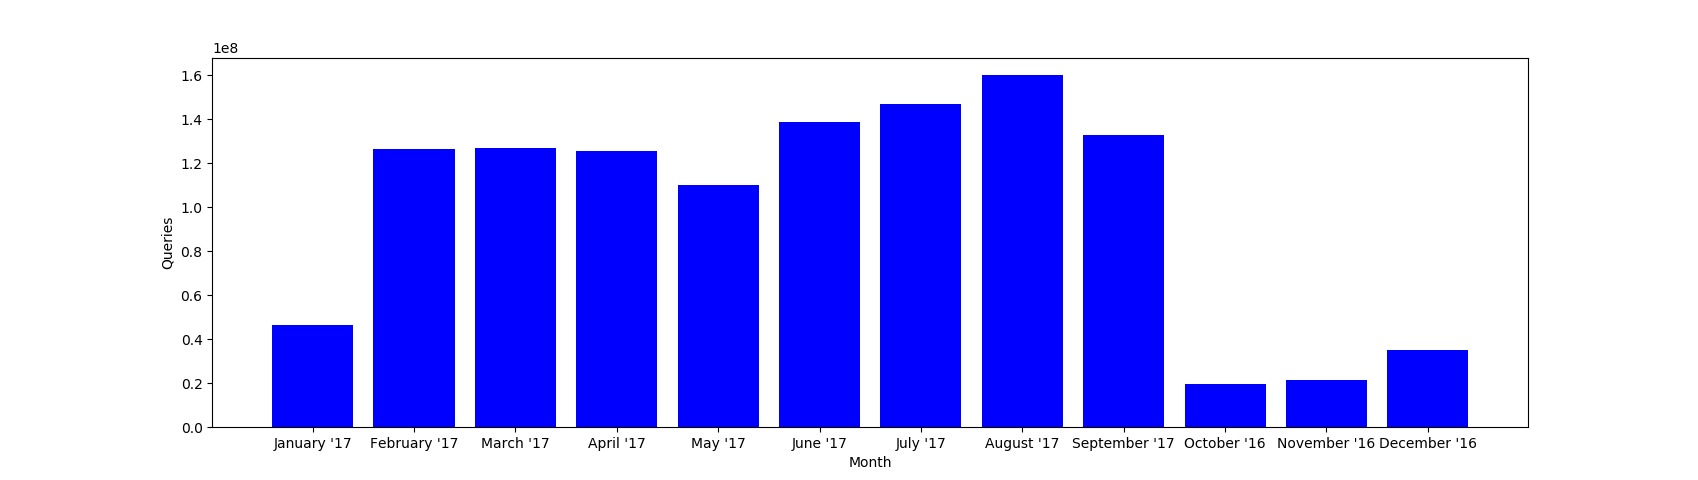
\includegraphics[width=1.0\textwidth]{images/liczba_zapytan_w_miesiacach.png}
\caption{\label{fig:zapytaniaMiesiace} Liczba zapytań w poszczególnych miesiącach}
\end{figure}

\subsection{Liczba zapytań w poszczególnych dniach}
Pozwoliliśmy sobie także wykonać wykres pokazujący liczbę zapytań w poszczególnych dniach tygodnia (rys. \ref{fig:zapytaniaDni}). Zauważamy tutaj pewną prawidłowość, otóż najwięcej zapytań jest w weekend (prawdopodobnie dlatego, że użytkownicy mają wtedy najwięcej czasu na wyszukiwanie nowych rzeczy w serwisie), a ich liczba spada niemalże liniowo w ciągu tygodnia by w weekend znów gwałtownie wzrosnąć.
 
\begin{figure}[!ht]
\centering
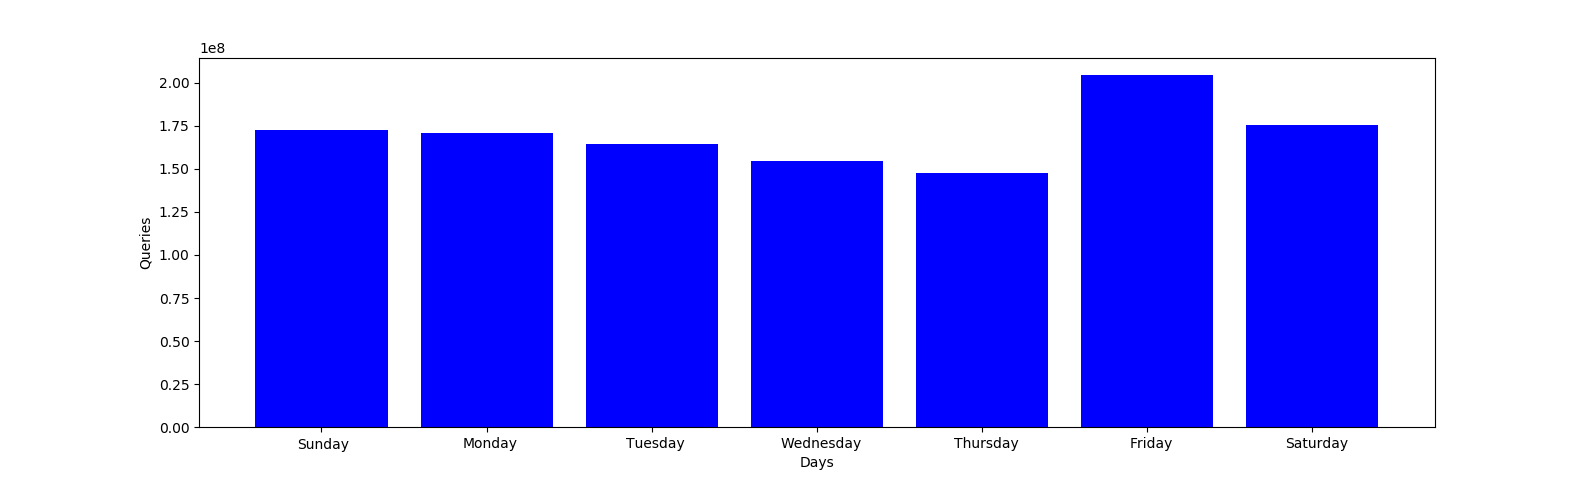
\includegraphics[width=1.0\textwidth]{images/liczba_zapytan_w_dniach_tygodnia.png}
\caption{\label{fig:zapytaniaDni} Liczba zapytań w poszczególnych dniach tygodnia}
\end{figure}

\section{Sprzedaż dla wybranych kategorii}
W niniejszym rozdziale opisaliśmy wykres dotyczących sprzedaży w wybranej przez nas kategorii.

\subsection{Histogram sprzedanych samochodów}

Rysunek \ref{fig:sprzedaneSamochody} prezentuje liczbę sprzedanych samochodów w poszczególnych miesiącach. Podobnie jak na poprzednich wykresach, tutaj również mieliśmy problemy z wczytaniem danych za niektóre miesiące. W związku z tym pominęliśmy cały styczeń. Ze względu na bardzo niewiele zapytań w okresie luty-kwiecień możemy stwierdzić, że mało osób kupuje samochody na początku roku. Obserwujemy tutaj, że liczba zapytań jest w miarę wyrównana w ciągu roku (z wyjątkiem wspomnianego wcześniej okresu). Od września do listopada notujemy pewien wzrost liczby wyszukiwań, która trochę spada w ostatnim miesiącu.

\begin{figure}[!ht]
\centering
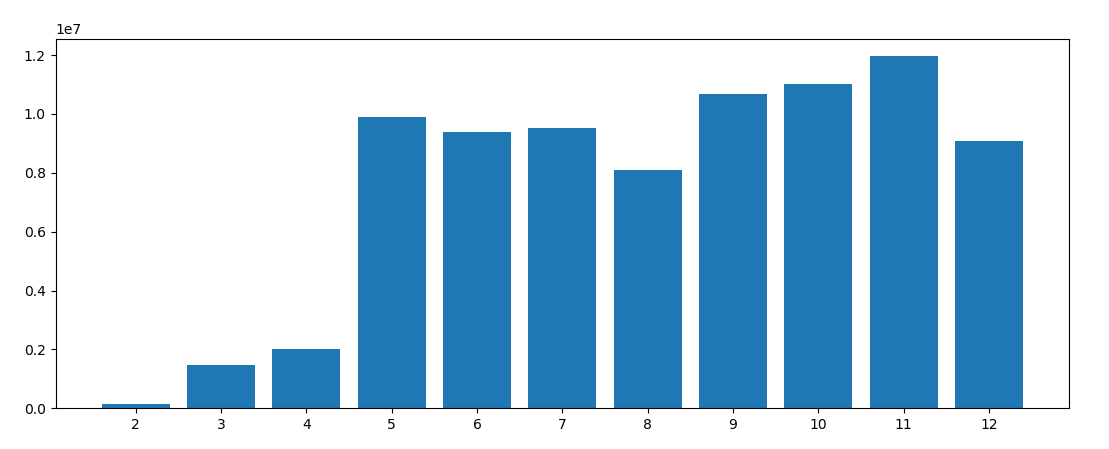
\includegraphics[width=1.0\textwidth]{images/sprzedane_samochody.png}
\caption{\label{fig:sprzedaneSamochody} Liczba zapytań w poszczególnych dniach tygodnia}
\end{figure}

\section{Podsumowanie}
Zauważyliśmy, że istnieją pewne korelacje pomiędzy liczbą sprzedaży, a liczbą wyszukiwań. Korelacja ta jest jednak dla nas trochę zaskakująca gdyż spodziewaliśmy się raczej, że zwiększenie się liczby zapytań spowoduje wzrost sprzedaży tymczasem jest odwrotnie. Wstępna analiza danych niestety nie odpowiedziała na wiele naszych pytań. Wciąż mamy mnóstwo wątpliwości. Na pewno będziemy jeszcze nie raz dokładnie przyglądać się danym.

\end{document}  